\documentclass[12pt]{report}

\usepackage[utf8]{inputenc}
\usepackage[french]{babel}
\usepackage[T1]{fontenc}
\usepackage{longtable}
\usepackage{graphicx}
\usepackage{verbatim} 
\usepackage{hyperref}
\usepackage{lastpage}
\usepackage{listings}

%-------------------------------------------------------------------------------------------------------------------------------
% Marges
\usepackage[top=2cm, bottom=2cm, left=2cm, right=2cm]{geometry} 
%-------------------------------------------------------------------------------------------------------------------------------

%-------------------------------------------------------------------------------------------------------------------------------
% Entete et pied de page
\usepackage{fancyhdr} 
\fancypagestyle{plain}{%
	\fancyhf{} 
	\fancyhead{}                  
	\fancyfoot{}   
	\fancyfoot[L]{Ufwi}
	\fancyfoot[C]{\thepage \/ \pageref{LastPage}}
	\fancyfoot[R]{\today}
	\chead{Projet tuteuré – Ufwi}
	\renewcommand{\headrulewidth}{1pt}   
	\renewcommand{\footrulewidth}{1pt}      
}
\pagestyle{plain}
%-------------------------------------------------------------------------------------------------------------------------------




%-------------------------------------------------------------------------------------------------------------------------------
% Gestion de l'affichage des chapitres
\makeatletter
\renewcommand{\@chapapp}{}
\makeatother
%-------------------------------------------------------------------------------------------------------------------------------

\title{Ufwi}
\author{Simon BAROTTE, Valentin FROLICH, Cyril PIERRÉ, Maxime ROBIN}
\date{\today}

\begin{document}



%-------------------------------------------------------------------------------------------------------------------------------
% Page d'accueil
\thispagestyle{empty}
\begin{center}
Licence Professionnel ASRALL


\vspace{1cm}
Projet tuteuré.

\vspace{2,5cm}

\begin{center}
  
\includegraphics[width=10cm,height=10cm]{images/ufwi.png}
\end{center}

\vspace{1cm}
\textbf{\Huge Ufwi}


\end{center}

\vspace{4cm}

Groupe :
\begin{itemize}
  \item Simon BAROTTE
  \item Valentin FROLICH
  \item Cyril PIERRÉ
  \item Maxime ROBIN
\end{itemize}


%-------------------------------------------------------------------------------------------------------------------------------

\newpage

%-------------------------------------------------------------------------------------------------------------------------------
% Sommaire
\renewcommand{\contentsname}{Sommaire}
\tableofcontents
%-------------------------------------------------------------------------------------------------------------------------------

\newpage

%-------------------------------------------------------------------------------------------------------------------------------
% Content
\chapter{Introduction}
\section{Historique}
Il faut savoir que le projet Ufwi descend du projet NuFW.
La première version publique de NuFW est sortie le 01 septembre 2003.L’idée avait germée en 2001 mais ne s’était concrétisée que le 01 septembre de l’année 2003.
La société croît rapidement, créant une vingtaine d'emplois en région parisienne, et acquérant une réputation dans le milieu de la sécurité informatique. 
En 2009, l'entreprise décide d'abandonner le pôle service pour se concentrer sur l'édition d'un pare-feu clef en main, EdenWall, couplant NuFW avec une interface d'administration performante.
Cette action entraîna des difficulté financiere lourde a la société.
Le 18 août 2011, soit sept ans après sa création, le tribunal du commerce de Paris a prononcé la liquidation de la société, et de se fait, la fin du projet NuFW.\\
Cependant le projet fut reprit sous le nom de Ufwi, offrant une reprise optimale du projet en opérant un rassemblement du code,
 notamment éparpillé chez les clients de la société, qui évite les mois de travail nécessaires à la récupération des modifications ayant eu lieu depuis cette date.
\section{Présentation}
Ufwi est une solution de pare-feu par authentification, cela signifie qu'il effectue une authentification de chaque connexion qui le traverse.
 L'authentification se fait de façon transparente, en requérant les informations d’identification via l'annuaire des utilisateurs d'un réseau (LDAP par défaut).
 Donc avec Ufwi chaque utilisateur doit décliner son identité à chaque initialisation de conexion. Une fois que l'utilisateur est identifié,
 le paquet se voit filtré, selon les droits associés à l'utilisateur.
 Une fois que le premier paquet est accepter, les paquets suivant appartenant à la même connexion sont gérés par le système de suivi d'état
 (seul le paquet d'initialisation d'une connexion est authentifié). Ce principe de fonctionnement requiert la présence d'un client sur le poste utilisateur, il existe des clients compatible pour windows et GNU/Linux.
Ufwi dispose aussi d'un mode sans client, pour se faire ufwi utilise un module "ufwi-authd" (utilisé dans le cadre de notre projet).\\
Comme vu précedemment Ufwi, chaque connexion est associée à un utilisateur. Ce qui veut dire que plusieurs utilisateurs peuvent travailler sur un même poste génèrent simultanément des flux à partir d'une même adresse IP source.

\newpage
Donc Ufwi permet le filtrage par utilisateur mais peut aussi apporter d'autre fonctionalité interessantes.\newline
\begin{itemize}
    \item Ufwi permet de contribuer de manière très pointue à la surveillance de l'activité réseau des serveurs. En regle générale dans les installations moderne on attribue des utilisateurs distinct à chaque service que fait tourner le serveur, de ce faite avec Ufwi on peut attribuer une politique réseau différente pour chaque utilisateur système.\newline
    \item Ufwi peut marquer chaque paquets d'une connexion avec les information de son utilisateur (identifiant...) ce qui permet d'appliquer une politique de qualité corespondant a chaque utilisateurs. Cela permetd onc de distribuer la bande passante en tre chaque utilisateur, ainsi attribuer une bande passante plus élevé au utilisateur qui utilise desn applications plus gourmande en terme de connexion.\newline
    \item Ufwi comprend un module de surveillance qui journalisent les événement principaux se produisant sur le réseaux en indiquant les utilisateurs à l'orgine de ses flux ( ouverture, fermeture de connexion, paquet bloqué, etc...). Ces log peuvent etre gérés au choix par Syslog, PostgreSQL ou MySQL. Ufwi conserve chaque connexion ouverte ( ou tenté) meme si l'utilisateur en question a changé d'adresse IP ou de machine.\newline
    \item Ufwi permet d'identifier les utilisateurs des aplications réseau grace a une authentification unique (Single sign on). Grace au systeme de journalisation Sql une table de connexion est maintenu en temps reel.  
%-------------------------------------------------------------------------------------------------------------------------------
\chapter{Liste des solutions de pare-feu par identification}
Les pare-feu par identifications les plus connus : 
  \begin{itemize}
    \item AuthPF : Fonctionne sous OpenBSD et qui se repose sur SSH pour l'identification des utilisateurs : http://www.openbsd.org/faq/pf/authpf.html
    \item NuFW : projet ayant donné naissance à UFWI suite à la liquiditation de l'éditeur "EdenWall Technologies"
    \item Cyberoam : pare-feu entièrement basé sur l'identification, en utilisant une corrélation entre adresse MAC et utilisateur : http://www.cyberoam.com/fr/firewall.html
    \item CheckPoint (NAC Blade) : utilisation des règles de filtrage en fonction d'une authentifcation basée sur Kerberos, l'identité de son poste et du niveau de sécurité du poste ( mise à jour de sécurité / antivirus ) : http://www.cyberoam.com/fr/firewall.html
    
  \end{itemize}
\begin{longtable}{|p{4cm}|p{6cm}|p{6cm}|}
  \hline
  \textbf{Solution parefeu} & \textbf{Avantage} & \textbf{Inconvégnient}\\
  \hline
    Ufwi &
     \begin{itemize}
        \item Projet devenu libre.
        \item Appliquer des règles horaires strictes.
        \item  composé de deux démons qui peuvent être mis en place sur des systèmes différents et le démon principal est massivement multithreadé.
        \item Contrôle d’accès sont réalisées grâce à des greffons (des modules system, ldap, dbm, plaintext).
        \item Journalisation de l’activité des utilisateurs peut être faite par syslog, mysql, postgresql.
        \item Multi plate-forme.
        \item Géneration des acl grace a un module (nuaclgen)
    \end{itemize}&
    \begin{itemize}
        \item Tres peu de documenation voir aucune (obligé de cf. à nufw).
        \item Nécessite une partie cliente spécifique sur les postes clients.
        \item Payante sous windows (NuWinC).
        \item Projet peu soutenu (temps de reponse 20-30 jours).
    \end{itemize} \\
  \hline
    AuthPF&
    \begin{itemize}
        \item règles par système et/ou par utilisateur.
        \item Connection via SSH.
        \item chaque utilisateur peut disposer de ses propres règles, présentes dans HOME/.authpf/authpf .rules.
        \item Simple a metre en place.
        \item  C'est un Firewall de type filtre de paquet (Couches réseau et transport).
        \item Documentation et suport en français et assez simple.
    \end{itemize}&
    \begin{itemize}
        \item l'utilisateur se déconnecte, le pare-feu lui retire les règles ajoutées.
        \item quelqu'un d'autre peut toujours spoofer cette IP et passer.
        \item Necessite la creation d'un home pour chaque utilisateur.
        \item Necessite Openbsd et des conaissance PF.
    \end{itemize} \\
  \hline
    Cyberoam&
    \begin{itemize}
        \item Sécurise les connexions IP dynamiques (Wi-Fi) et les postes de travail partagés.
        \item Les politiques basées sur l'identité de l'utilisateur permettent d'éviter les erreurs rencontrées avec les politiques basées sur les adresses IP.
        \item Prend en charge la création de groupes en fonction du profil professionnel sur l'ensemble des sites distribués.
    \end{itemize}&
    \begin{itemize}
        \item 
        \item 
    \end{itemize} \\
  \hline
    CheckPoint&
    \begin{itemize}
        \item Permet définitions de politique granulaires par utilisateur et de groupe.
        \item L'intégration transparente avec Active Directory.
        \item Idéal pour la protection des environnements avec les médias sociaux et des applications Internet.
    \end{itemize}&
    \begin{itemize}
        \item 
        \item 
    \end{itemize} \\
    \hline
\end{longtable}
\newligne
%-------------------------------------------------------------------------------------------------------------------------------

%-------------------------------------------------------------------------------------------------------------------------------
\chapter{Fonctionnement d'ufwi}
\section{Algorithme}

\begin{enumerate}
  \item Au démarrage de sa session de travail, l’utilisateur lance un client sur son poste de travail. Le client ouvre un tunnel crypté par TLS vers le serveur nuauth qui réalise l’authentification de l’utilisateur pour ce tunnel au regard d’un annuaire référent. Ce tunnel est ensuite conservé pendant toute la durée des opérations et l’ensemble des échanges entre nuauth et le client se fait ensuite par son intermédiaire.
  \\
  \item Supposons maintenant que l’utilisateur ouvre une connexion vers un serveur, par exemple une connexion web à destination du serveur d’application. Il utilise alors son navigateur favori qui envoie un paquet à destination du serveur. Le paquet envoyé est un paquet TCP standard avec notamment comme caractéristiques port destination 80 (web) et bit SYN positionné (ouverture de connexion).
  \\
  \item Le pare-feu (Netfilter) envoie ce paquet au démon nufw (au moyen de la décision QUEUE ou NFQUEUE) : contrairement à un pare-feu " classique ", Netfilter ne prend pas de décision à propos de cette connexion.
  \\
  \item Le démon nufw se contente de relayer le paquet reçu vers le serveur d’authentification, qui a autorité sur les décisions.
  \\
  \item Le démon nuauth analyse le paquet reçu (et en particulier l’adresse IP source) et envoie une demande de mise à jour à tous les clients connectés (par l’étape 1) depuis cette adresse pour qu’ils authentifient les connexions en attente. Cette demande est envoyée au travers du (ou des) canal (canaux) crypté(s) ouvert(s) à l’étape 1.
  \\
  \item Le client qui a ouvert notre connexion " témoin " stipule à nuauth qu’il l’a fait, en précisant tous les paramètres IP (IP et port destination, port source, etc.). À ce stade, le serveur nuauth connaît, de manière sûre, l’identité de l’utilisateur à la source de notre connexion.
  \\
  \item nuauth réalise une requête sur la base des ACL, pour vérifier si l’utilisateur dispose des droits pour établir cette connexion. nuauth obtient ainsi une décision.
  \\
  \item (En option) nuauth journalise toutes les informations relatives à cette connexion dans une base SQL, avec bien sûr l’identité de l’utilisateur.
  \\
  \item nuauth envoie la décision obtenue en 7 à nufw, qui la relaie à son tour à Netfilter. La décision associée à notre utilisateur est alors appliquée par Netfilter.
  \\
  \item S’il est autorisé, le paquet poursuit sa route.
  \\
  \item (En option) Si le serveur (Apache, par exemple) désire connaître l’identité de l’utilisateur, au lieu de la lui demander directement, il peut réaliser une simple requête SQL SELECT pour récupérer l’identifiant de l’utilisateur en partant de marqueurs uniques de la connexion (la socket source, pour les connaisseurs). L’utilisateur est ainsi authentifié de manière transparente, et sans pouvoir tricher, sur le serveur : il s’agit d’une solution de Single Sign On (authentification unique) très simple, très sûre, et indépendante du protocole.
  \\
  \item Le reste du flux est géré par le suivi de connexion (Stateful inspection) de Netfilter : les paquets ne repassent pas par les démons nufw/nuauth.
\end{enumerate}
\begin{center}
  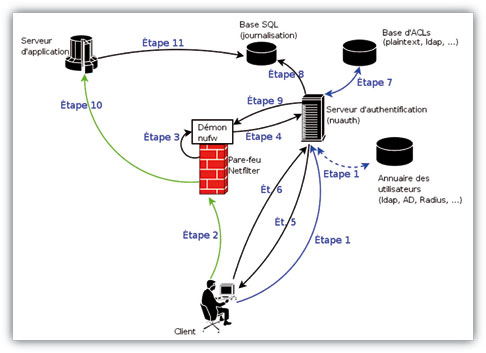
\includegraphics[width=12cm,height=10cm]{images/algo.jpg}
\end{center}

%-------------------------------------------------------------------------------------------------------------------------------
\chapter{Daemon ufwi-authd}
\section{Introduction}

Nuauth command est une interface qui permet de contrôler des fonctions importantes du daemon authd, 
comme l'obtention de la liste des utilisateurs connectés par exemple.
Chaque fois qu'un client envoie un paquet(1) pour commencer une connexion à travers la 
passerelle, la station cliente envoie un paquet(2) d'identification au daemon authd. Le 
pare-feu de la passerelle met en file d'attente le paquet et envoie directement des 
informations au daemon authd.

Le travail du daemon va être d'analyser les deux paquets (1) et (2) et de vérifier si 
le client à le droit d'initialiser la connexion qu'il demande.
Si ufwi-authd indique que le paquet(1) est autorisé alors la connexion est initialisé,
sinon la connexion est annulé. Ufwi-authd peut aussi utiliser un serveur LDAP pour la
définition des utilisateurs et groupes.

Ci-dessous le un schéma montrant le processus d'authentification utilisé par NuFW, resté inchangé avec UFWI:

\begin{center}
  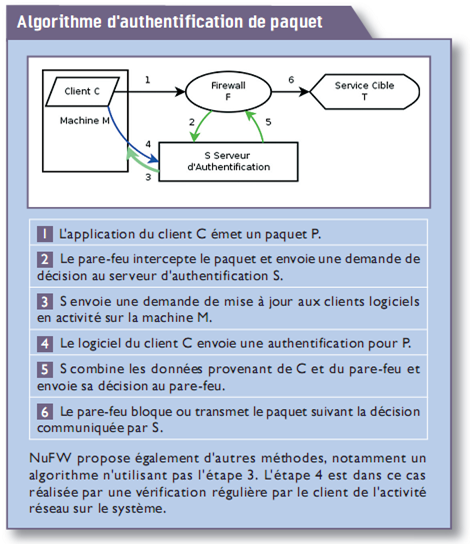
\includegraphics[width=8cm,height=10cm]{images/auth.png}
\end{center}

\section{Intallation}

Pré-requis :

Script autogen.sh :
    \begin{itemize}
      \item version automake1.7
    \end{itemize}
Compilation Nufw :
  \begin{itemize}
    \item GNU libtool
    \item GNU make
    \item libpam-dev
    \item glib 2.4+
    \item libipq (iptables-dev pour debian) ou libnetfilter queue
    \item libldap
    \item libsasl2
    \item libgnutls
    \item libgcrypt
  \end{itemize}

Noyau:

Il est recommandé d'utiliser un noyau récent afin de bénificer de toutes les dernières nouveautés implémenter dans ce dernier.
Une version de noyau supèrieur à 2.6.18 est un bon choix. Le patch dump-connection-mark.diff ( disponible dans patches/ ) 
peut être appliqué au noyau afin d'améliorer les perfomances de ce dernier lorsque nous utiliserons le log de session.

Compilation:

La compilation du daemon est relativement simple, elle se déroule en quatre étapes:
  \begin{itemize}
   \item Lancement du script ./autogen.sh
   \item Exécution de ./configure
   \item make
   \item Et pour finir make install
  \end{itemize}
Lors de la première installation, il faut penser à copier le ficheir de configuration avec la commande suivante:

\textit{cp ./conf/nuauth.conf /usr/local/etc/nuauth.conf}

\section{Sécuriser l’installation}
\subsection{Vérification des certificats}
Il est particulièrement recommandé de placer nuauth dans un endroit protégé afin de garantir la sécurité
des communications entre nufw et nuauth\footnote{Même si tous les paquets sont chiffrés par TLS}. 
Dans la mesure où la décision du pare-feu dépend de la réponse de nuauth, il est important de pouvoir 
valider l’identité du serveur nuauth. Pour cela, on peut demander à nufw de vérifier le certificat présenté 
par nuauth lors de l’établissement du tunnel TLS. Ceci peut être mis en place grâce à l’option -a suivie du nom 
du fichier contenant le certificat d’autorité racine. Cette option est ajoutée à la ligne de commande démarrant nufw. 
Ce faisant, nufw vérifiera la validité du certificat présenté par nauth.

\subsection{Côté client}
Du côté du client, le système doit être intègre pour que les informations conernant les applications et le
système d’exploitation soient pertinentes. On doit toujours garder à l’esprit que seul l’agent installé
côté client est capable d’obtenir ces renseignements. En cas d’attaque, il est évident que ces informations
PEUVENT et SERONT faussées par l’installation d’un agent NuFW modifié.

On doit tenir compte de cet avertissement et ne surtout pas oublier que cette
fonctionnalité permet de sécuriser des flux qui auraient dû être ouvert sans vérification sur un système
basique.

La pertinence du filtrage d’application et/ou de système d’exploitation dépend de la confiance que l'on
place dans le système qui réalisera l’authentification. Elle est "relativement bonne" sur un système
sécurisé sur lequel les utilisateurs ne peuvent installer de logiciels

\section{Quelques commandes liées au daemon}

Commandes principales:
\begin{itemize}
  \item quit: déconnexion
  \item refresh cache: rafraichit tous les caches
  \item reload: recharge la configuration du daemon d'authentification 
\end{itemize}
Information:
\begin{itemize}
  \item help: affiche la liste des commandes utilisables
  \item version: affiche la version du daemon
  \item uptime: affiche depuis combien de temp tourne le daemon 
\end{itemize}
Gestion des utilisateurs:
\begin{itemize}
  \item users: affiche els utilisateurs connectés
  \item disconnect all: déconnecte tous les utilisateurs
  \item disconnect ID: déconnecte un utilisateur grâce à son identifiant (ID) 
\end{itemize}

\section{Fichier de configuration}

Le fichier authd.conf est le fichier principal de configuration pour le
daemon ufwi-authd. C'est dans ce fichier que seront indiqué l'adresse du daemon ufwi-filterd 
par exemple ou encore le niveau de debug, le nombre de connexion qu'un utilsateur peut lancer.
Dans ce fichier seront aussi renseigné les différents paramètres qui guide le comportement du 
daemon, mais aussi les paramètres système, et pour finir les chemins absolus des autres fichiers
de configuration.

Il existe aussi d'autres fichiers de configurations liés à ufwi-authd:
\begin{itemize}
  \item modules/nuauth-tls.conf qui contiendra les paramètres TLS
  \item modules/nuauth-krb5.conf configuration authentification Kerberos 5
  \item modules/nuauth-ldap.conf authentification ldap
  \item modules/nuauth-mysql.conf configuration de la base de donnée pour les logs utilisateurs (mysql)
  \item modules/nuauth-pgsql.conf configuration de la base de donnée pour les logs utilisateurs (postgres) 
\end{itemize}
 
\section{Installation des certificats}

Le daemon d'authentification et le client utilise des certificats afin de comuniquer ensemble. Lors de l'installation de la
suite ufwi des certificats sont installés par défaut dans le répertoire /certs. On peut utiliser ces certificats par défaut 
pour procéder à des tests mais il n'est pas conseillé de les utiliser pour un utilisation pro de la suite ufwi. Dans cette 
section nous allons voir comment générer ces certificats.

Génére notre propre Authorité de Certification:

\textit{mkdir private}

\textit{chmod 700 private}

\textit{openssl req -new -x509 -keyout private/CAkey.pem -out private/CAcert.pem}

Génére les clefs privées pour le client et le daemon d'authentification:

\textit{openssl genrsa -out private/nufw-key.pem}

\textit{openssl genrsa -out private/nuauth-key.pem}

Génére les demandes de certificats pour le client et le daemon:

\textit{openssl req -new -key private/nufw-key.pem -out nufw.csr}

\textit{openssl req -new -key private/nuauth-key.pem -out nuauth.csr}

Signe les demandes de certificats grâce à l’AC:

\textit{openssl x509 -req -days 365 -in nufw.csr -CA private/CAcert.pem -CAkey private/CAkey.pem -CAcreateserial -out nufw-cert.pem}

\textit{openssl x509 -req -days 365 -in nuauth.csr -CA private/CAcert.pem -CAkey private/CAkey.pem -CAcreateserial -out nuauth-cert.pem}
\\
Enfin on déplace les certificats dans le bon répertoire:

\textit{cp private/nufw-key.pem /etc/nufw/}

\textit{cp nufw-cert.pem /etc/nufw/}

\textit{cp private/nuauth-key.pem /etc/nufw/}

\textit{cp nuauth-cert.pem /etc/nufw/}

\section{Configuration basique du daemon}

Lors de l'installation de la suite ufwi un fichier de configuration de base est fournie nuauth.conf, qui est disponible 
dans le répertoire conf.
Ce fichier est remplie de plusieurs directives, les deux plus importantes directives de configuration sont : 
nuauth client listen addr : qui définit l’adresse à laquelle le daemon va attendre les requètes des clients 
nuauth nufw listen addr : qui définit l’adresse à laquelle le daemon va attendre les requètes de nufw. 
La liste des machines autorisées à se connecter au serveur d'authentifcation constitue la variable nufw gw addr.

Ensuite, on doit choisir le module d’authentification et de vérification des ACL. Les modules suivants sont disponibles :
\begin{itemize}
 \item libldap : les informations utilisateur sont stockées dans un annuaire LDAP
 \item dbm : les informations utilisateur sont stockées dans une base gdbm
 \item plaintext : les informations utilisateur sont stockées dans un fichier texte
 \item system : l’authentification s’adosse à PAM et utilise les groupes existants dans le système. Ceci procure un 
moyen pratique d’utiliser nss et/ou pam-modules
\end{itemize}

Le module d’authentification est paramétrable via l’option nuauth user check module dont la valeur par défaut est
libsystem (si non défini dans le fichier de configuration). D’autre paramètres concernant la vérification
des ACL doivent être précisés si on choisit une des deux authentification suivante :
\begin{itemize}
 \item libldap
 \item plaintext
\end{itemize}
Tout ceci en définissant la variable nuauth acl check module.

 \section{Procédure de test}
Lors du projet nous avons installé une machine virtuelle avec l'iso nufw pré-installées.
Détail des configurations effectuées :
\subsection{Paramétrage Iptables}
Tout d'abord mise en place de règles Iptables de façon à déclencher une 
demande d’authentification pour toute connection vers ssh:

\textit{iptables -A OUTPUT -s 192.168.1.0/24 -p tcp --dport 22 -m state --state NEW --syn -j NFQUEUE}

\textit{iptables -A OUTPUT -m state --state ESTABLISHED,RELATED -j ACCEPT}

\subsection{Test du système d’authentification}
Nous avons laissé la configuration par défaut de nuauth.

\textit{nuauth -vvvvvvvvv} (les v en argument corresponde au niveau de debug du daemon, ici niveau 9, niveau
max)

Ensuite, on démarre nufw dans un autre terminal, avec ici aussi le niveau de debug max afin d'avoir
le plus d'informations possible sur le daemon.

\textit{nufw -vvvvvvvvv}

Enfin, on peut essayer de connecter un utilisateur. On utilise nutpc pour réaliser ceci avec
 la commande :

\textit{nutcpc -d -H [NUAUTH IP]} ou NUAUTH IP correspond à l'adresse IP de la machine qui exécute nuauth.

Dans le terminal qui exécute nuauth :

\textit{user simon@nufw uses OS Linux, 3.0.10, #1 Tue Mar 19 23:00:32 CEST 2012}

Cette ligne nous donne le nom de l'utilisateur qui se connecte, ici simon, l'OS utiliser par 
cette utilisateur ainsi que la date et l'heure.

\subsection{Déroulement de l'authentification}
La connection SSH va déclencher la procédure d’authentification :
\begin{itemize}
	\item nufw reçoit un paquet de Netfilter :
		\subitem [PID] Sending request for 3352783904
	\item nufw ouvre une connexion TLS vers nuauth :
		\subitem [PID] Trying TLS connection
	\item nuauth reçoit la requète de nufw :
		\subitem ** Message: Packet :
		\subitem ** Message: Connection : src=192.168.1.12 dst=192.168.1.12 proto=6
		\subitem ** Message: sport=32848 dport=22
	\item nuauth envoie une demande d’authentification au client en fonction de l’IP source :
		\subitem ** Message: need to warn client
		\subitem ** Message: sending request
	\item nuauth reçoit la réponse du client :
		\subitem ** Message: User :
		\subitem ** Message: Connection : src=192.168.1.12 dst=192.168.1.12 proto=6
		\subitem ** Message: sport=32848 dport=22
		\subitem ** Message: OS : Linux 2.6.9 #1 Fri Mar 16 21:51:32 CEST 2012
		\subitem ** Message: Application : /usr/bin/ssh
	\item nuauth renvoie sa réponse à nufw :
		\subitem Sending auth answer 1 for 3352783904 on 0x42428482 ...
	\item nufw renvoie le paquet dans le noyau :
		\subitem [PID] Accepting 3352783904
\end{itemize}

Remarque:

Ne JAMAIS nutcpc avec l’adresse [NUAUTH IP] égale à localhost ou 127.0.0.1, même si nuauth 
est installé sur la même machine. Dans ce cas, les paquets envoyés à nuauth 
par le pare-feu proviendront de la machine (avec une adresse égale à, par exemple,
192.168.0.1) alors que nuauth attend pour l’authentification une adresse égale à 127.0.0.1. 
Dès lors, l’authentification échouera systématiquement.

\subsection{Utilisation du module LDAP}
Après avoir réalisé un test de base de nuauth, vous avons tenter l'utilisation de LDAP pour vérifier les comptes d'utilisateurs. Malgrès l'échec 
de cette configuration nous explicitons notre démarche : 
acls.schema dans le répertoire \textit{/etc/ldap/schema} et ajout de la ligne suivante dans le fichier \textit{/etc/ldap/slapd.conf} : 
\textit{include  /etc/ldap/schema/acls.schema}.

Configuration de nuauth (nuauth.conf) pour l'utilisation de LDAP comme suit:

Modification de la directive nuauth\_acl\_check\_module pour lui indiquer l'utilisation de libldap.

Ensuite, préciser les paramètres de connexion à l’annuaire :

\textit{ldap\_bind\_dn="uid=nuauth,ou=Users,dc=inl,dc=fr"}

\textit{ldap\_bind\_password="secretpassword"}

\textit{ldap\_basedn="dc=inl,dc=fr"}

\textit{ldap\_acls\_base\_dn="ou=Acls,dc=inl,dc=fr"}

\section{Suivi des connexions avec SQL}
Configuration de nuauth pour permettre le suivi des connexions grâce à une base de données SQL. Pour commencer pour 
activer le suivi de connexion avec NuFW, nous avons paramétré les options suivantes dans le fichier nuauth.conf :

\textit{nuauth\_log\_users\_sync=1}

\textit{nuauth\_log\_users=8}

Pour journaliser en MySQL, il faut avoir une base contenant la bonne structure. Pour ce faire on peut utiliser 
le fichier nulog.mysql.dump du répertoire conf et les commandes suivantes (dans un terminal) :

\textit{mysqladmin create nulog}

\textit{cat conf/nulog.mysql.dump|mysql nulog}

Il suffit ensuite de créer un utilisateur MySql qui aura les droits SELECT, DELETE, UPDATE et INSERT sur la table. Enfin, ajoute 
les informations de connexions au serveur SQL dans le fichier nuauth.conf, en modifiant les directives suiventes:

\textit{mysql\_server\_addr="localhost"}

\textit{mysql\_server\_port="3306"}

\textit{mysql\_user="nuauth"} (ici c'est le nom que nous avons donné à l'utilisateur SQL)

\textit{mysql\_passwd="root"}

\textit{mysql\_table\_name="nulog"} (ici on renseigne le nom de la table crée ci-dessus)

Après différente recherche sur la journalisation des connexions avec SQL nous avons trouvé une discussion d'utilisateur, 
cette discussion avait pour sujet l'utilisation d'un script clean\_conntrack.pl qui est disponnible dans le répertoire scripts 
à partir de la version 1.0.12. 
Ce script doit être exécuté très régulièrement, à intervalles de quelques minutes seulement, par l’intermédiaire de cron, 
notamment en cas de trafic important.La seule opération réalisée par le script est de transférer les connexions "mortes" 
(ie les connexions fermées ou refusées) vers une autre table, qui sera une table d’archivage.Il faut envisager d’archiver 
régulièrement la table d'archivage, afin d’éviter qu’elle ne grossisse indéfiniment.

\section{Authentification par fichier locale}
Il existe un autre moyen de spécifier des utilisateurs à nuauth. Nuauth considère que la base des utilisateurs est locale, 
dans un fichier plat, ce type de configuration est très simple à mettre en place, et est donc parfait pour réaliser des tests.
Tout d'abord il va falloir vérifier quelques options importantes de notre configuration nuauth, dans 
\textit{/etc/nufw/nuauth.conf}.

\textit{nuauth\_user\_check\_module="plaintext"}

C'est grâce à cette directive que nuauth va savoir que nous utilisons un fichier plat. 
Bien sûr, sur un réseau d’entreprise, on interface plutôt nuauth à l’annuaire (LDAP, Active Directory, Radius, etc.)

\textit{nuauth\_acl\_check\_module="libplaintext"}

Cette directive indique à nuauth de chercher les droits de chaque utilisateur dans un fichier texte également.

À présent, on crée notre fichier texte de définition des utilisateurs \textit{/etc/nufw/users.nufw} avec le contenu suivant.

\textit{simon:simon:1:102}

\textit{admin:iadmin:2:100,102}

\textit{suadmin:suroot:3:103}

Le fichier définit donc trois utilisateurs : simon, admin et suadmin. Le deuxième champ (après le " : ") est 
le mot de passe. Le troisième champ est un identifiant propre à chaque utilisateur. Enfin, le dernier champ définit la 
liste des groupes (numériques) auxquels l’utilisateur appartient. Ici, donc, l’utilisateur simon a comme mot de passe simon, 
comme identifiant 1 et appartient au groupe 102.

Bien évidemment, ces utilisateurs sont totalement indépendants des utilisateurs systèmes existants sur le pare-feu. 
Notre base d’utilisateur est ici parfaitement spécifique à NuFW. Voyons à présent les ACL. Nous allons créer le 
fichier \textit{/etc/nufw/acls.nufw} avec le contenu suivant :

\textit{[http]}

\textit{#1 = acceptation, 0 = rejet}

\textit{decision=1}

\textit{# groupes concernés par cette décision}

\textit{gid=102}

\textit{# L’identifiant du protocole, tel que décrit par /etc/protocols. Ici il s’agit de TCP == 6}

\textit{proto=6}

\textit{SrcIP=0.0.0.0/0}

\textit{SrcPort=1024-65535}

\textit{DstIP=192.168.1.12}

\textit{DstPort=80}

Ici on autorise donc les membres du groupe 102 à surfer sur le site web de la machine 192.168.1.12. Dans notre exemple, 
il s’agit des utilisateurs simon et admin.

Recharge la configuration du serveur nuauth:

\textit{killall -HUP nuauth}

à présent, lançe le client :

\textit{nutcpc -H IP\_nuauth -U user}

Si tout se passe bien, le mot de passe concernat l'user choisit est demandé. Pour tester il suffirait de faire un simple
telnet sur la machine 192.168.1.12 sur le port 80 et vérifier que la connexion s'ouvre bien.


%-------------------------------------------------------------------------------------------------------------------------------
\chapter{Daemon ufwi-filterd}
\section{Introduction}

	Le daemon ufwi-filterd (ancienement appelé nufw) n'est d'autre qu'un pare-feu basé sur NFQUEUE netfilter. Il permet d'écrire des règles de filtrage basées sur l'identité des utilisateurs, en plus des critères de réseau classiques. L'authentification effectue de façon transparente en requérant les informations d’identification de l’utilisateur avantqu’une quelconque décision de filtrage ne soit prise. En pratique, cela signifie que les politiques defiltrage peuvent intégrer l’annuaire utilisateur, et amène cette notion d’ID utilisateur au niveau de la couche IP.\\
Ufwi-filterd est capable de:
\begin{itemize}
  \item Filtrer le trafic en fonction du système d’exploitation et des applications utilisées par les utilisateurs
     distants.
  \item marquer chaque paquet d'une connexion avec l'identifiant de son utilisateur et donc d'appliquer une politique de qualité de service spécifique à chaque utilisateur. 
  \item contribue de manière très pointue à la surveillance de l'activité réseau des serveurs.
  \item dispose de modules de surveillance qui journalisent les événements principaux de l'activité du réseau en indiquant quels sont les utilisateurs à l'origine des flux.
\end{itemize}
\section{Intallation}
Une installation typique de la suite logicielle NuFW comporte 2 démons : nufw (ufwi-filterd) et nuauth (ufwi-authd) et autant de clients que nécessaire.\\
Pré-requis :
\begin{itemize}
  \item automake1.7 pour executer autogen.sh
  \item GNU libtool
  \item GNU make
\end{itemize}
Pré-requis pour la compilation et l'excution de ufwi-filterd :
\begin{itemize}
  \item ufwi-base
  \item ufwi-confparser
  \item ufwi-ssl
\end{itemize}
Il est recommandé d'utiliser un noyau récent afin de béneficer de toutes les dernières nou-
veautés implémenter dans ce dernier. Une version de noyau supèrieur à 2.6.18 est un bon choix.
\newpage
\section{Compilation}
La compilation de ufwi-filterd est relativement simple elle se resume a utiliser les commandes suivantes :
\begin{itemize}
  \item ./autogen.sh
  \item ./configure
  \item make
  \item makeinstall
\end{itemize}
Lors de la première installation, il ne faut pas oublier de copier le fichier de configuration "make install-conf" afin de chercher les changements entre votre fichier de conf actuelle et le nouveau.\\
Un fichier INSTALL avec toutes les instructions a suivre est fournie dans le dossier de ufwi-filerd disponible a partir de se lien http://ufwi.org/projects/ufwi-filterd/ repository .
\section{Commandes}
Tout dabord, vous devez executer en root ufwi-filterd.
ufwi-filterd -h vous donnera un message d'aide pour l'utilisation de ufwi-filterd.
\section{Fichier de configuration}
Le fichier de configuration de ufwi-filterd se nome tout simplement "filterd.conf". On poura le trouver dans /etc/ufwi-filterd/.
Dans se fichier on trouvera l'adresse ou le nom du serveur d'authentification nuauth (par defaut 127.0.0.1), on trouvera aussi les chemin absolut des fichiers :
\begin{itemize}
  \item /etc/ufwi-filterd/key.pem (clé privé du serveur)
  \item /etc/ufwi-filterd/cert.pem (certificat du serveur)
  \item /etc/ufwi-filterd/cacert.pem
  \item /etc/ufwi-filterd/crl.pem (liste de révocation de certificat serveur)
\end{itemize}

%-------------------------------------------------------------------------------------------------------------------------------
\chapter{Daemon ufwi-rcpd}
\section{Introduction}
Le module ufwi-rcpd (anciènnement appelé NuCentral) est le module qui gère les autres deamons.

\section{Installation}
\subsection{Pré-requis}
Avant de lancer l'installation du module, certains pré-requis sont nécéssaires :
\begin{itemize}
  \item Python 2.5
  \item Twisted web
  \item M2Crypto
  \item Jinja
  \item Subversion (svnadmin program)
  \item sudo
  \item pysvn
  \item pytz
\end{itemize}
Debian: \begin{verbatim}apt-get install python-twisted-web python-svn 
    python-m2crypto sudo python-jinja subversion python-tz\end{verbatim}
\newline

Pour l'installation de ufwi-rpcd:
\begin{itemize}
  \item (GNU) make
  \item sqlite3
\end{itemize}
Sous Debian: \begin{verbatim}apt-get install make sqlite3\end{verbatim}
\newline

Paquets optionnels :
Pour compiler les fichiers de .ts à .qm et mettre à jours les transmissions :
\begin{itemize}
  \item lrelease4: Qt development tools
  \item pylupdate4, lrelease-qt4: Python Qt development tools
\end{itemize}
Sous Debian: \begin{verbatim}apt-get install libqt4-dev pyqt4-dev-tools\end{verbatim}
\newline

Autres :
\begin{itemize}
  \item python-twisted-snmp : pour le module SNMP.
  \item gnutls-bin : le programme certtool l'utilise pour générer les certificats ssl.
  \item py.test (Sous Debian, python-codespeak-lib) : utilisé pour les tests.
  \item libconfig-inifiles-perl : pour tools/ufwi\_rpcd\_enmod.
  \item IPy (python-ipy) : pour les tests.
\end{itemize}

\section{Utilisation}
Une fois démarrer, on peut accèder au fonction plus particuliaire de ufwi-rpcd (nucentral).
\subsection{Démarrage}
\subsubsection{Lancement en mode deamon}
Pour lancer ufwi-rpcd en mode deamon il suffit d'exécuter une commande en root:
\begin{verbatim}
twistd -y /usr/sbin/ufwi-rpcd.tac --pidfile=/var/run/ufwi-rpcd.pid 
    -l /var/log/ufwi-rpcd-twisted.log
\end{verbatim}
   
Pour arrèter ufwi-rpcd en mode deamon (en root):
\begin{verbatim}kill \$(cat /var/run/ufwi-rpcd.pid)\end{verbatim}
   
\subsubsection{Lancement en mode "premier plan"}
Pour facilité le développement, on peut également lancer ufwi-rpcd en premier plan:
\begin{verbatim}twistd -n -y /usr/sbin/ufwi-rpcd.tac -l /var/log/ufwi-rpcd-twisted.log\end{verbatim}
Pour arréter le processus : CTRL+c.

\subsection{ufwi\_rpcd\_client (nucentral\_client)}
\subsubsection{Le client}
Pour lancer le client d'ufwi\_rpcd en HTTP (tcp/8080):
\begin{verbatim}ufwi_rpcd_client --host 127.0.0.1 --cleartext -u admin -p admin\end{verbatim}
Par défaut, ufwi\_rpcd\_client utilise HTTPS (tcp/8443):
\begin{verbatim}ufwi_rpcd_client --host 127.0.0.1 -u admin -p admin\end{verbatim}
Une fois connecté sur le client, le prompt devient: 
\begin{verbatim}nucentral>\end{verbatim}

\subsubsection{Le menu}
Une fois lancer, on peut accèder aux différentes fonctions d'ufwi-rpcd:
\begin{itemize}
  \item \begin{verbatim}call('component', 'service', ...)\end{verbatim}
  Apelle un service d'NuCentral
  \item \begin{verbatim}authenticate('login', 'password')\end{verbatim}
  Authentification ou mise à jour d'un groupe ou d'un utilisateur.
  \item \begin{verbatim}components()\end{verbatim}
  Affiche la liste des différents composants.
  \item \begin{verbatim}services('component')\end{verbatim}
  Affiche la liste des services d'un composant.
  \item \begin{verbatim}proxy('component')\end{verbatim}
  Créé un composant pour le proxy qui pourra être utilisé avec component.service().
  \item \begin{verbatim}nucentralStatus()\end{verbatim}
  Afficher l'état du serveur et la session d'informations.
  \item \begin{verbatim}help('component')\end{verbatim}
  Utilisation d'un composant.
  \item \begin{verbatim}help('component', 'service')\end{verbatim}
  Utilisation d'un service d'un composant.
  \item \begin{verbatim}help(proxy)\end{verbatim}
  Utilisation du proxy.
  \item \begin{verbatim}exit()\end{verbatim}
  Quitter.
  \item \begin{verbatim}pyhelp(object)\end{verbatim}
  Aide Python pour l'objet spécifié.
  
\end{itemize}
\\
\\
Différents composants sont disonibles :
\begin{verbatim}
CORE, access, acl, audit, auth_cert, bind, config, contact, hostname, hosts, 
httpout, localfw, lock, logger, network, ntp, nuauth, nuauth_command, nuconf, 
nuface, nulog, nupki, nurestore, reporting, resolv, session, status, streaming, 
system, system_info, tools, update, users_config, versionning
\end{verbatim}


%---------------------------------------------------------------------------------------------------------------------------------
\chapter{Client Ufwi/nufw}
Comme vu précedemment dans l'intruductuin Ufwi a besoin d'une partit client sur chaque poste utilisent ce logiciel. Cependant il y'a un moyen de contourné se probleme sous 
GNU/Linux.\\ Il est possible de s'authentifier directement au serveur UFWI au moment de l'authentification de l'utilisateur sur un poste linux.
Pour cela, il est nécessaire d'installer le paquet pam\_nufw présent dans la plupart des distributions GNU/Linux. Il est possible de trouver les sources de ce logiciel dans les sources du projet NuFW.
Pour configurer, il suffit de renseigner la ligne suivante dans /etc/pam.d/common-auth :
\begin{verbatim}
	auth optional pam_nufw.so server=adresse_amon port=4129 noauth=root,mdp
\end{verbatim}
et dans /etc/pam.d/common-session :
\begin{verbatim}
	session optional pam_nufw.so server=adresse_amon port=4129 noauth=root,mdp
\end{verbatim}
Un client graphique autonome est proposé librement par la société INL. Ce client, NuApplet2, est disponible dans la plupart des distributions GNU/Linux.
L'adresse IP correspond à l'amon et le port correspond au service Nuauth (4129 par défaut).\newligne
\vspace{1,5cm}
\begin{center}
  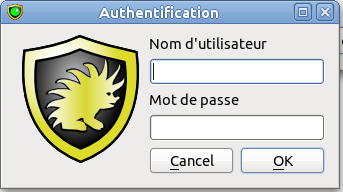
\includegraphics[width=5cm,height=4cm]{images/nuapp.png}
\end{center}
\vspace{1,5cm}
UN autre client exicte sous GNU/Linux Nutcpc celui ci est celui que nous avons utilisé pour nos test, c'est un client non-graphique uniquement en ligne de commande. Ce client est le client de base proposé dans l'iso de Nufw. Le client a besoin de certificat d'authentification SSL, pour les configurer deux solution sont disponible. La premiere (recommandé) est de mettre directement les certificats d'authentification dans le dossier c'est a dire dans le /home/user/.nufw . La deuxieme solution consisitant a definir les certificats d'hautentification en parametre de la commande.\\
Quelque commande pour le client nutcpc :
\newpagge
\begin{itemize}
	\item -h : Affiche les differente commande.
	\item -v : Affiche la version du client.
	\item -d : affiche le mode debug.
	\item -S : utilise le SSL pour se connecter auserveur Nuauth.
	\item -k : Avant de demarre, le programe rue tout les processus existant de l'userID
	\item -l : ne verifie pas les lokfile avant de demarrer et n'en créé pas.
	\item -H + Ip serveur Nuauth : Envoie un packet d'authentification au serveur.
	\item -p + port du serveur Nuauth : Envoie un packet d'authentification au serveur (port).
	\item -U : Definie l'utiliastauer (UserID).
	\item -P : Set le mot de passe utilisateur.
	\item -C : Define le certfile qui autorise la connection TLS a Nuauth.
	\item -A : Definie l'AuthorityFile et verifie la validité des certificats de Nuauth.
	\item -k : Définei la KeyFile qui autorise la connection TLS.
\end{itemize}
\vspace{0,7cm}
Un exemple typique pour tester si le client dialogue bien avec le serveur est de faire:
\begin{verbatim}
	nutcpc -d 9 -H 192.168.1.137 -A Nuauth_cert.pem
\end{verbatim}
Donc dans la commande ci dessus on active le mode debug avac le plus haut niveau pour plus d'info en cas de probleme ou d'erreure, ensuite on configure l'IP du serveur Nuauth et enfin on definie le certificats si il n'est pas deja placé dans .nufw de l'utilisateur et verifie la validité des certificats de Nuauth.
\vspace{0,7cm}
Il existe toutefois un client nufw pour windows non libre pour le moment. NuWinC est le client NuFW pour les OS de microsoft, Windows.Le client NuWinC est intégré au client Scribe mais il est désactivé par défaut.Avant tout, il faut activer le client NuWinC. Cela se fait dans ESU.Après l'avoir activé, il faut paramétrer l'IP de l'Amon et le port du serveur d'authentification Nuauth (4129).
\begin{center}
  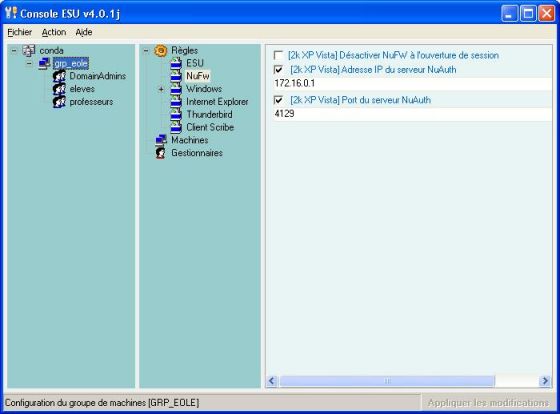
\includegraphics[width=7cm,height=6cm]{images/nuwinc.png}
\end{center}
\newpage
ESU permet de régler certains paramètres spécifiques à NuWinC.Il est, par exemple, possible de protéger ou de masquer le client NuFW.
\begin{center}
  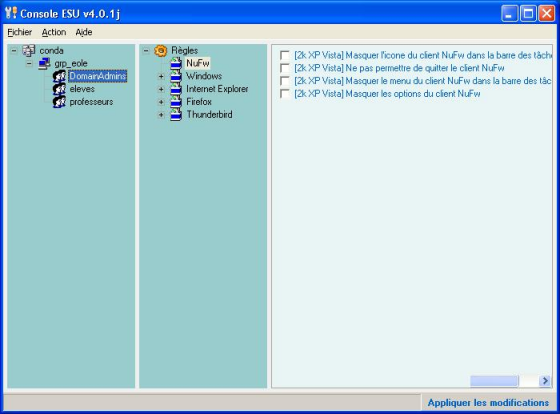
\includegraphics[width=7cm,height=6cm]{images/nuwinc1.png}
\end{center}
%---------------------------------------------------------------------------------------------------------------------------------
\chapter{Externalisation des logs dans une BD MySQL}
\underline{Configuration du serveur BD}
\newline
Installation des paquets :
\newline

apt-get install apache2 php5 mysql-server nulog
\newline

\underline{Configuration de la passerelle :}
\newline

Configuration IP :
\newline

ifconfig eth0 192.168.1.137/24
\newline
ifconfig eth1 172.20.8.1/24
\newline

Installation des paquets :
\newline

apt-get install ulogd ulogd-mysql
\newline

Correction d'un bug : ajout d’une ligne dans le script de démarrage qui va charger un module
\newline

nano /etc/init.d/ulogd
\newline
export LD_PRELOAD=/usr/lib/libmysqlclient.so.16
\newline

Configuration de ulogd : modification de son fichier de configuration
\newline

nano /etc/ulogd.conf
\newline

Décommenter la ligne 46 (pour charger un module supplémentaire)
\newline

Renseigner les informations de connexion à la base de données :
\newline

paragraphe « [MYSQL] » ligne 59 :
table=’’ulog’’
pass=’’passulog’’
user=’’ulog’’
db=’’ulog’’
host=’’172.20.8.2’’

\newline
Configuration du serveur de BD:
\newline

Configuration IP :
\newline

ifconfig eth0 172.20.8.2/24
\newline

Lister tous les fichiers installés à l’installation de nulog :
\newline

dpkg –L nulog | more
\newline

Ouvrir le fichier suvant (démarche à suivre pour creer les tables de la base de données)
\newline

nano /usr/share/doc/nulog/README.Debian
\newline

Connexion à la base de données et création de l’utilisateur (les deux programmes vont se connecter avec ce compte):
\newline

mysql –u root –p
create database ulog;
create user 'ulog'@'\%' identified by 'passulog' ;
grant all privileges on ulog.* to ulog;
exit
\newline

Commandes de création de la base :
\newline

cd /usr/share/doc/nulog/scripts
gunzip ipv4.sql.gz
cat ipv4.sql | mysql –uulog –p ulog

\newline
Modification du fichier de configuration de mysql
\newline

nano /etc/mysql//my.cnf
ligne 47
\newline

Il faut qu’il écoute sur l’interface 172.20.8.2

bind address= ‘’172.20.8.2’’
\newline

Renommer les fichiers de configuration :
\newline

cd /etc/nulog
cp default. core.conf core.conf
cp default.nulog.conf nulog.conf
cp default.wrapper.conf wrapper.conf
\newline

Renseigner les informations de connexion à la base de données :
\newline

nano core.conf
host=localhost
db=ulog
user=ulog
password=passulog
table=ulog

\newline
Prise en compte des changements : redémarrage de services
Sur la passerelle :
\newline

/etc/init.d/ulogd restart

\newline
Sur le serveur :

\newline
/etc/init.d/ulogd restart


On choisit ce que l’on veut loguer avec iptables

%---------------------------------------------------------------------------------------------------------------------------------
\chapter{Difficulté rencontré et avis personnel}
\section{Daemon d'authentifcation}
\subsection{Problèmes rencontrés}
Au début du projet, nous avons voulu installer UFWI sur une distribution Debian afin de pouvoir tester les modules PyQT qui fonctionnent en GUI,
alors que l'iso NUFW ne fonctionne qu'en CLI.
À ce moment du projet, aucune documentation technique n'était disponible pour l'installation du logiciel.
Nous avons donc télécharger l'ensemble des modules qui composent UFWI et avons testé l'installation "à l'aveugle" sans savoir quelles étaient les 
dépendances entre ces différents modules.
De plus un grand nombre de dépendance n'étaient pas satisfaites car UFWI exigeait des librairies trop anciennes pour fonctionner, 
certaines de ces librairies n'étant plus disponible sur une debian stable.
En fonction des modules il fallut même utiliser des versions différentes d'autogen.
Nous avons ensuite découvert un bug dans "UFWI Base", 
lors de l'installation du module ufwi-base, le make génère un src/MakeFile contenant une erreur : 
l'installation avec make install appelle deux fois successivement le script security.h ce qui retourne un message d'erreur. 
Il faut donc éditer le MakeFile généré et supprimé le deuxième security.h pour que l'installation fonctionne correctement :

fichier base/src/MakeFile
ligne 223 :
include_HEADERS = linuxlist.h config-table.h ipv6.h log.h ufwibase.h packet_par$
security.h debug.h documentation.h jhash.h ufwi_source.h proto.$
proto_v3.h proto_v4.h proto_v5.h security.h

Ce bug a été rapporté au support UFWI et a été corrigé récemment : http://www.ufwi.org/issues/65#change-8

Mais lorsqu'enfin tout les modules sont installés il est impossible de les lancer, d'autres dépendances étant manquantes.
Nous avons donc utiliser une nouvelle iso de projet nufw qui venait d'être mis en ligne pour pouvoir enfin tester le logiciel.


\subsection{Avis personnel}


Ce projet tuteuré a tout de même été une bonne expériences, malgrès "l'echec" de l'utilisation de ce logiciel. 
Nufw peut être très puissant et réellement utile pour une entreprise. Une fois que ce logiciel fonctionne il est assez 
simple de l'utiliser, le seul problème réel problème étant la jeunesse du projet (très peu de documentation ont été mise en ligne par exemple).

Un point particulièrement intéressant durant ce projet, fût de découvrir un bug d'installation qui nous a permit de légèrement contribuer au projet.

%---------------------------------------------------------------------------------------------------------------------------------
\chapter{Planning}
\textbf{Maxime Robin :}
\begin{itemize}
  \item Semaine 4 à 8 (Du 23 janvier au 27 février) :
  \begin{itemize}
    \item Mise en place du dépot github.
    \item Étude et installation du deamon ufwi-rpcd.
    \item Commencement du rapport.
  \end{itemize}
  \item Semaine 9 :
  \begin{itemize}
    \item Étude de la durée de vie des autorisations données.
  \end{itemize}
  \item Semaine 10 et 11 :
  \begin{itemize}
    \item Installation de l'ISO de NuFW dans une machine virtual disponnible sur le site de nufw.
    \item Mise en place sur le réseau de la nouvelle machine.
    \item Étude des fonctions préinstallées sur la nouvelle machine préinstaller.
  \end{itemize}
  \item Semaine 12 :
  \begin{itemize}
    \item Étude des différentes fonctions du module nucetral (ufwi-rpcd).
  \end{itemize}
\end{itemize}

\textbf{Simon Barotte :}
\begin{itemize}
  \item Début janvier :
  \begin{itemize}
    \item Etude du daemon ufwi-auth.
    \item Installation du daemon (sans succès)
  \end{itemize}
  \item Mois janvier début février :
  \begin{itemize}
    \item Rédaction de la partie ufwi-auth du rapport
    \item Etude des erreurs lors de la tentative d'installation du daemon
  \end{itemize}
  \item Mis février début mars :
  \begin{itemize}
    \item Etude des commandes du daemon ufwi-auth après le succès de l'installation
  \end{itemize}
  \item Mars :
  \begin{itemize}
    \item Prise en main de mon daemon (ufwi-auth)
	  \item Mettre en place différent test et valider leur fonctionnement
	  \item Utiliser différentes configuration en tirer les avantages et inconvénients
	  \item Générer des certificats personnel pour nuauth	
	  \item Test du système d'authentification
	  \item Réaliser premier test et débogage
  \end{itemize}
\end{itemize}
	
\textbf{Valentin Frolich :} 
\begin{itemize}
  \item Semaine 4 à 7 :
  \begin{itemize}
    \item Etude du daemon Ufwi-filtred.
	  \item Ecriture de la partie Daemon Ufwi-filtred du rapport.
	  \item Etude des prerequis et dependance pour l'instalation de la suite Ufwi.
  \end{itemize}
  \item Semaine 9 :
  \begin{itemize}
    \item Rédaction de la partit Introduction du rapport.
  \end{itemize}
  \item Mars :
  \begin{itemize}
    \item Tester different configuration de la suite Ufwi.
	  \item Simuler un environement test (entreprise...).
	  \item Definir les limite, avantage, inconvénient de la suite.
  \end{itemize}
\end{itemize}

\textbf{Cyril PIERRÉ :}
\begin{itemize}
  \item Semaine 4 à 8 :
  \begin{itemize}
    \item Mise en place d'un réseau virtualisé à l'aide de VirtualBox comprenant une passerelle	entre le réseau ASRALL (192.168.1.0/24) et le réseau interne virtuel (172.20.8.0) et d'une seconde machine avec un annuaire LDAP, un serveur MySQL et un serveur de résolution DNS (bind9)
	  \item Étude des PyQT Managements Tools
	  \item Installation de l'ensemble des modules d'UFWI sur la passerelle
	  \item Recherche des différents pare-feu par authentification
	  \item Mise en place d'un tutoriel pour l'externalisation des logs de pare-feu avec Nulog
  \end{itemize}
  \item Semaine 9 :
  \begin{itemize}
    \item Correction d'un problème de RAM sur la passerelle
	  \item Étude de l'intégration d'UFWI avec d'autre logiciels d'authentification :
	  \begin{itemize}
      \item Kerberos
    \end{itemize}
  \end{itemize}
\end{itemize}
\end{document}
